%%%%%%%%%%%%%%%%%%%%%%%%%%%%%%%%%%%%%%%%%%%%%%%%%%%%%%%%%%%%%%%%%%%%%%%%%%%%%%%%%%
\begin{frame}[fragile]\frametitle{}
\begin{center}
{\Large GST FAQ Chatbot}


{\tiny (Ref: Building a FAQ Chatbot in Python – The Future of Information Searching - Yogesh Kulkarni)}

{\tiny https://www.analyticsvidhya.com/blog/2018/01/faq-chatbots-the-future-of-information-searching/}
\end{center}
\end{frame}

%%%%%%%%%%%%%%%%%%%%%%%%%%%%%%%%%%%%%%%%%%%%%%%%%%%%%%%%%%%
 \begin{frame}[fragile]\frametitle{Introduction}
\begin{itemize}
\item What do we do when we need any information? Simple: ``We Ask, and Google Tells''.
\item But if the answer depends on multiple variables or changes as per context, then the existing Ask-Tell model tends to sputter.
\item Solution: Chatbots.
\end{itemize}
\end{frame}


%%%%%%%%%%%%%%%%%%%%%%%%%%%%%%%%%%%%%%%%%%%%%%%%%%%%%%%%%%%
 \begin{frame}[fragile]\frametitle{Introduction to GST Chatbot}
\begin{itemize}
\item Goods and Services Tax (GST) was recently introduced in India (2017)
\item A lot of people are still trying to understand how it works. 
\item Chatbots can provide such information in a natural and conversational way.
\end{itemize}
\end{frame}

%%%%%%%%%%%%%%%%%%%%%%%%%%%%%%%%%%%%%%%%%%%%%%%%%%%%%%%%%%%
 \begin{frame}[fragile]\frametitle{FAQs better with Chatbots}
\begin{itemize}
\item To know more about GST, like how to apply for registrations, tax slabs, etc., there are many Frequently Asked Questions (FAQs) on different websites. 
\item Going through that amount of information can be a painstaking process. 
\item In these situations, chatbots come in handy, effective and thus, have become enormously popular.
\end{itemize}
\end{frame}

%%%%%%%%%%%%%%%%%%%%%%%%%%%%%%%%%%%%%%%%%%%%%%%%%%%%%%%%%%%
 \begin{frame}[fragile]\frametitle{GST FAQ bot architecture}
\begin{itemize}
\item A chatbot is a client-server application. 
\item In the case of RASA-NLU, even the server can be local. 
\item The client is nothing but the chabot UI.
\end{itemize}
\end{frame}

%%%%%%%%%%%%%%%%%%%%%%%%%%%%%%%%%%%%%%%%%%%%%%%%%%%%%%%%%%%
 \begin{frame}[fragile]\frametitle{GST FAQ bot architecture}
The interaction and architecture can be understood by the following diagram:

\begin{center}
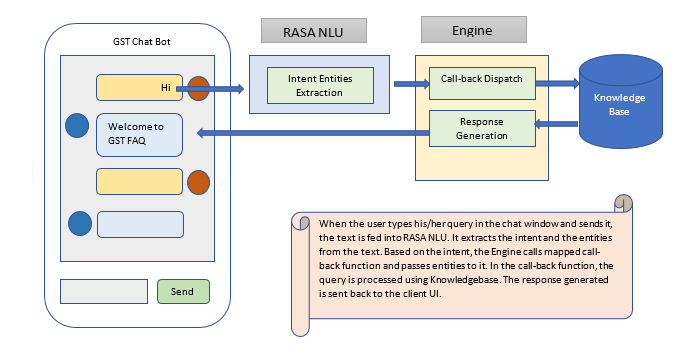
\includegraphics[width=\linewidth,keepaspectratio]{gstbot1}
\end{center}

\end{frame}

%%%%%%%%%%%%%%%%%%%%%%%%%%%%%%%%%%%%%%%%%%%%%%%%%%%%%%%%%%%
 \begin{frame}[fragile]\frametitle{Steps to build server side of the GST chat bot application}
 \begin{itemize}
\item Create a new directory and navigate to it.
\item Create the following things in it:
\begin{itemize}
\item nlu\_data directory
\item nlu\_data/gstfaq-data.json: This has GST FAQ training examples as shown above
\item nlu\_config.yml: This has settings for RASA-NLU as shown below:
\begin{lstlisting}
{
  pipeline: spacy_sklearn,
  language: en
}
\end{lstlisting}
\end{itemize}
\end{itemize}
\end{frame}

%%%%%%%%%%%%%%%%%%%%%%%%%%%%%%%%%%%%%%%%%%%%%%%%%%%%%%%%%%%
 \begin{frame}[fragile]\frametitle{Training}
\begin{itemize}
\item Train the model in python. Write a script ``run\_training.bat'' like below
\begin{lstlisting}
python -m rasa_nlu.train -c nlu_config.yml -d nlu_data/gstfaq-data.json  --path projects --verbose
\end{lstlisting}
\item What do these parameters mean?

\begin{itemize}
\item config: configuration of the machine learning model
\item data: file / folder that contains the training data
\item path: output path where the model is persisted to
\end{itemize}
\item Model will be created in a new folder ``projects/default/model\_YYYYMMDD-HHMMSS''
\end{itemize}
\end{frame}

%%%%%%%%%%%%%%%%%%%%%%%%%%%%%%%%%%%%%%%%%%%%%%%%%%%%%%%%%%%
 \begin{frame}[fragile]\frametitle{Extract Intent and Entities}
\begin{itemize}
\item There are two ways you can use your model, directly from python, or by starting a http server. Details of running the Rasa NLU HTTP server are in config.
\item To use your new model in python, create an Interpreter object and pass a message to its parse() method:
\begin{lstlisting}
from rasa_nlu.model import Interpreter
import json
interpreter = Interpreter.load(".projects/default/model_YYYYMMDD-HHMMSS")
message = "let's see some italian restaurants"
result = interpreter.parse(message)
print(json.dumps(result, indent=2))
\end{lstlisting}
\end{itemize}

\end{frame}

%%%%%%%%%%%%%%%%%%%%%%%%%%%%%%%%%%%%%%%%%%%%%%%%%%%%%%%%%%%
 \begin{frame}[fragile]\frametitle{HTTP server}
\begin{itemize}
\item For starting HTTP server, create and run following script ``run\_server.bat''
\begin{lstlisting}
python -m rasa_nlu.server --path projects
\end{lstlisting}
\item This starts the RASA-NLU server and let us know the port
\item By default, the server will look for all projects folders under the path directory specified. 
\item When no project is specified, as in this example, a ``default'' one will be used, itself using the latest trained model.
\end{itemize}
\end{frame}



%%%%%%%%%%%%%%%%%%%%%%%%%%%%%%%%%%%%%%%%%%%%%%%%%%%%%%%%%%%
 \begin{frame}[fragile]\frametitle{Testing}
\begin{itemize}
\item Once the server starts running you can GET/POST via curl to post or use it as the HTTP server
\item Then, in the browser, type: http://localhost:5000/parse?q=hello%20there
\item Another way: For windows users the windows command line interface doesn’t like single quotes. Use doublequotes and escape where necessary.
\begin{lstlisting}
curl -X POST localhost:5000/parse -d ``{"q":"I am looking for Mexican food"}'' | python -m json.tool
\end{lstlisting}
\end{itemize}
\end{frame}

%%%%%%%%%%%%%%%%%%%%%%%%%%%%%%%%%%%%%%%%%%%%%%%%%%%%%%%%%%%
 \begin{frame}[fragile]\frametitle{Response Json}
The output is shown below:
\scriptsize
\begin{lstlisting}
{
  "entities": [],
  "model": "model_20181001-113701",
  "intent": {
    "confidence": 0.4157846092697248,
    "name": "affirm"
  },
  "text": "hello there",
  "project": "default",
  "intent_ranking": [
    {
      "confidence": 0.4157846092697248,
      "name": "affirm"
    },
    {
      "confidence": 0.32066813872253364,
      "name": "greet"
    },
    :
  ]
}
\end{lstlisting}
\begin{itemize}
\item Rasa NLU will also print a confidence value for the intent classification. 
\item For models using spacy intent classification this will be a probability.
\end{itemize}
\end{frame}

%%%%%%%%%%%%%%%%%%%%%%%%%%%%%%%%%%%%%%%%%%%%%%%%%%%%%%%%%%%
 \begin{frame}[fragile]\frametitle{Client}
 Our chatbot client UI has been built using Flask framework. It uses two html templates to render the UI (i.e. the chat window). 
 The outer UI is built with base.html as shown below:
 \tiny
\begin{lstlisting}
<!DOCTYPE HTML>
<html lang=''en''>
<head>
...
</head>
    <body>
         <h1 align="center">GST FAQ Chat</h1>
        <div class="container">
            
        </div>
</body>
    <footer>
        
    </footer>
</html>
\end{lstlisting}
\end{frame}

%%%%%%%%%%%%%%%%%%%%%%%%%%%%%%%%%%%%%%%%%%%%%%%%%%%%%%%%%%%
 \begin{frame}[fragile]\frametitle{Client}
The content and other\_footers blocks are defined in home.html as shown below:
\tiny
\begin{lstlisting}

<div class="row">
    <div class="col-sm-6">
        <div class="row">
            <div class="chat_window">
                <ul class="messages"></ul>
                <div class="bottom_wrapper clearfix">
                    <div class="message_input_wrapper">
                        <input id="msg_input" class="message_input" placeholder="Say Hi to begin chat..." />
                    </div>
                    <div class="send_message">
                         <div class="text">send</div>
                    </div>
                </div>
            </div>
:
\end{lstlisting}
\end{frame}

%%%%%%%%%%%%%%%%%%%%%%%%%%%%%%%%%%%%%%%%%%%%%%%%%%%%%%%%%%%
 \begin{frame}[fragile]\frametitle{Client}
The content and other\_footers blocks are defined in home.html as shown below:
\tiny
\begin{lstlisting}
:
            <div class="message_template">
                <li class="message">
                    <div class="avatar"></div>
                    <div class="text_wrapper">
                        <div class="text"></div>
                    </div>
                </li>
            </div>
        </div>
    </div>
</div>




<script src="{{ url_for('static', filename="js/bind.js") }}"></script>

\end{lstlisting}
\end{frame}


%%%%%%%%%%%%%%%%%%%%%%%%%%%%%%%%%%%%%%%%%%%%%%%%%%%%%%%%%%%
 \begin{frame}[fragile]\frametitle{Flask App}
The engine’s use of RASA-NLU for intent-entities extraction and dispatching call-backs can be seen below:
\scriptsize
\begin{lstlisting}
@app.route('/chat',methods=["POST"])
def chat():
    try:
        user_message = request.form["text"]
        response = requests.get("http://localhost:5000/parse",params={"q":user_message})
        response = response.json()
        response = response["topScoringIntent"]
        intent = response.get("intent")
        entities = response.get("entities")
        if intent == "gst-info":
            response_text = gst_info(entities
        elif intent == "gst-query":
            response_text = gst_query(entities)
        else:
            response_text = get_random_response(intent)
        return jsonify({"status":"success","response":response_text})
    except Exception as e:
        print(e)
        return jsonify({"status":"success","response":"Sorry I am not trained to do that yet..."})
\end{lstlisting}
\end{frame}

%%%%%%%%%%%%%%%%%%%%%%%%%%%%%%%%%%%%%%%%%%%%%%%%%%%%%%%%%%%
 \begin{frame}[fragile]\frametitle{GST Engine}
\begin{itemize}
\item This is the heart of the chatbot. 
\item Based on the intent received from RASA-NLU, it dispatches the entities to the mapped call-back functions. 
\item The function in turn, depending on the entities, calls Knowledgebase to get the response. 
\item Once the response is received, it is sent back to the UI.
\item Knowledgebase can be as simple as a dictionary of questions and answers, or as sophisticated as one can imagine/require (like databases, internet sources, etc.). 
\item This, being minimalistic for demonstration purposes, fetches pre-coded responses from the dictionary.
\end{itemize}

\end{frame}

%%%%%%%%%%%%%%%%%%%%%%%%%%%%%%%%%%%%%%%%%%%%%%%%%%%%%%%%%%%
 \begin{frame}[fragile]\frametitle{GST Engine}
 Let's take a look at the sample dictionary:

\scriptsize
\begin{lstlisting}
intent_response_dict = {
    "intro": ["This is a GST FAQ bot. One stop-shop to all your GST related queries"],
    "greet":["hey","hello","hi"],
    "goodbye":["bye","It was nice talking to you","see you","ttyl"],
    "affirm":["cool","I know you would like it"],
    "faq_link":['You can check all the events here <a href="https://www.cbec.gov.in/resources//htdocs-cbec/deptt_offcr/faq-on-gst.pdf</a>']
}
\end{lstlisting}
\end{frame}

%%%%%%%%%%%%%%%%%%%%%%%%%%%%%%%%%%%%%%%%%%%%%%%%%%%%%%%%%%%
 \begin{frame}[fragile]\frametitle{GST Engine}
\scriptsize
\begin{lstlisting}
gstinfo_response_dict = {
    "GST": " Goods and Service Tax (GST) is a destination based tax on consumption of goods and services.",
    "benefits":"GST consumes more than a dozen taxes, thus making it hassle free and efficient.",
    "faq_link":'You can check all the answers here <a href="http://www.cbec.gov.in/resources//htdocs-cbec/deptt_offcr/faq-on-gst.pdf</a>'
}

def gst_info(entities):
    if entities == None:
        return "Could not find out specific information about this ..." +  gstinfo_response_dict["faq_link"]
    if len(entities) == 1:
        return gstinfo_response_dict[entities[0]]
    return "Sorry.." + gstinfo_response_dict["faq_link"]
\end{lstlisting}
\end{frame}

%%%%%%%%%%%%%%%%%%%%%%%%%%%%%%%%%%%%%%%%%%%%%%%%%%%%%%%%%%%
 \begin{frame}[fragile]\frametitle{GST Engine}
\scriptsize
\begin{lstlisting}
gst_query_value_dict = {
    "12%":"Non-AC hotels, business class air ticket, frozen meat products, butter, cheese, ghee, dry fruits in packaged form, animal fat, sausage, fruit juices, namkeen and ketchup",
    "5%":"railways, air travel, branded paneer, frozen vegetables, coffee, tea, spices, kerosene, coal, medicines",
    "18%":"AC hotels that serve liquor, telecom services, IT services, flavored refined sugar, pasta, cornflakes, pastries and cakes",
    "28%":"5-star hotels, race club betting,wafers coated with chocolate, pan masala and aerated water",
    "exempt":"education, milk, butter milk, curd, natural honey, fresh fruits and vegetables, flour, besan"
}
def gst_query(entities):
    if entities == None:
        return "Could not query this ..." + gstinfo_response_dict["faq_link"]
    for ent in entities:
        qtype = ent["type"]
        qval = ent["entity"]
        if qtype == "gst-query-value":
            return gst_query_value_dict[qval]

        return gstinfo_response_dict[entities[0]]
    return "Sorry.." + gstinfo_response_dict["faq_link"]
\end{lstlisting}
\end{frame}

%%%%%%%%%%%%%%%%%%%%%%%%%%%%%%%%%%%%%%%%%%%%%%%%%%%%%%%%%%%
 \begin{frame}[fragile]\frametitle{GST Engine}
\begin{itemize}
\item User text is sent to the RASA-NLU server using http://localhost:5000/parse. 
\item Its response contains the intent and the entities. 
\item Depending on the intent, functions like gst-info and gst-query are called. 
\item Their responses are then sent back to the UI.
\end{itemize}
\end{frame}

%%%%%%%%%%%%%%%%%%%%%%%%%%%%%%%%%%%%%%%%%%%%%%%%%%%%%%%%%%%
 \begin{frame}[fragile]\frametitle{GST chatbot in action}
 Steps to operate:
\begin{itemize}
\item Start the RASA-NLU server by executing ``run\_server.bat'' script. It loads the custom trained model and starts listening to port 5000
\item Execute the Flash app, by running ``python app.py'' which starts flask server at localhost at port, say 8080.
\item Start typing commands in the bottom chat window and click ``Send''.
\item Typed messages and their responses appear in the window above
\end{itemize}
\end{frame}

%%%%%%%%%%%%%%%%%%%%%%%%%%%%%%%%%%%%%%%%%%%%%%%%%%%%%%%%%%%
 \begin{frame}[fragile]\frametitle{GST FAQ bot In Action}
\begin{center}
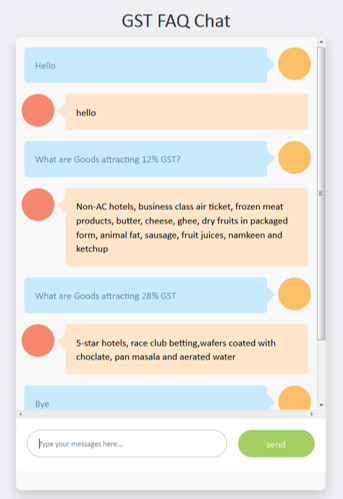
\includegraphics[width=0.35\linewidth,keepaspectratio]{GST-Bot1}
\end{center}
You can view the video demonstration at https://youtu.be/ct3eydFKYsg
\end{frame}


%%%%%%%%%%%%%%%%%%%%%%%%%%%%%%%%%%%%%%%%%%%%%%%%%%%%%%%%%%%
 \begin{frame}[fragile]\frametitle{End Notes}
\begin{itemize}
\item This presents just a small example, demonstrating the potential to develop something full-fledged and practically useful.
\item Our GST Q\&A bot can be enhanced on various fronts, such as expansion of knowledge-base (i.e. number of questions and answers), better training to find more intents and entities, Natural Language Generation of the responses to have a human language feel, etc.
\item GST FAQ Bot is just one example of building an intuitive front-end using government information. With the availability of more APIs and open public data, we can build similar (if not better) bots for those databases. Imagine interacting with government departments using a chatty bot!
\end{itemize}
\end{frame}